\documentclass[12pt,a4paper]{article}
\usepackage[utf8]{inputenc}
\usepackage[german]{babel}
\usepackage[T1]{fontenc}
\usepackage{amsmath}
\usepackage{amsfonts}
\usepackage{amssymb}
\usepackage{graphicx}
\usepackage{siunitx}
\usepackage{float}
\usepackage[left=2cm,right=2cm,top=2cm,bottom=2cm]{geometry}
\author{Gerald}

\begin{document}
\sisetup{separate-uncertainty = true}
	\setlength{\parindent}{0pt} 
	\begin{center}
		{\LARGE Versuchsprotokoll}\\
		\begin{large}
			zum Fortgeschrittenenpraktikum im Bachelorstudiengang Physik\\[0.4cm]
			an der RWTH Aachen\\
			II. Physikalisches Institut A\\[5.5cm]
			\Large\textbf{\textsl{Mößbauerspektroskopie (T05)}}\\[5.5cm]
			\normalsize\textit{vorgelegt\\von}\\[0.4cm]
			\large{Moritz Berger (355244)\\Gerald Kolter (355005)}\\\textbf{Gruppe 30}\\[2cm]
			\large \textbf{Wintersemester 2017/18}
		\end{large}
	\end{center}
	\newpage
	
	\tableofcontents
	\newpage

\section{Versuchsziel}
Das Ziel des Versuchs besteht darin, mithilfe der Mößbauerlinie folgende quantenmechanische Energieaufspaltungen von Eisen zu vermessen:
\begin{enumerate}
\item Die magnetische Hyperfeinstruktur
\item die elektrische Quadrupolaufspaltung
\end{enumerate}
Zudem soll das Einlinienspektrum von Eisen aufgenommen und der Extinktionswirkungsquerschnitt von Eisen, Stahl und Eisensulfat vermessen werden.

\section{Aufbau}
Der Aufbau zur Mößbauerspektroskopie besteht aus einer von einem Transducer in Strahlrichtung bewegten $^{57}$Co Quelle, einem Absorber und einem Detektor. Die Quelle sendet $\gamma$-Strahlung verschiedener Energie aus, wobei hauptsächlich die \SI{14,4}{keV} Linie betrachtet wird. Der Detektor zählt einzelne $\gamma$-Quanten innerhalb eines Energieintervalls, wobei 1024 Kanäle zur Verfügung stehen. Der Transducer bewegt die Quelle sinusförmig.

\section{Durchführung}

\begin{table}
\centering
\begin{tabular}{|c|c|}
\hline 
Spannung am Proportionalzählrohr & \SI{2}{kV} \\ 
\hline 
Messmodus & Pulshöhenanalyse (PHA-Modus) \\
\hline 
Messbereich im PHA-Modus & \SI{4,2}{V} - \SI{6,4}{V} \\
\hline 
\end{tabular} 
\caption{Allgemeine Messeinstellungen.}
\label{tab:Mess_Einstellungen}
\end{table}

Tabelle \ref{tab:Mess_Einstellungen} zeigt die verwendeten Messeinstellungen. Um bei für jede Messung den relevanten Energiebereich vermessen zu können, wurde die Transducer-Geschwindigkeit verändert. Die aus aus der Bewegung resultierende Dopplerverschiebung  ergibt eine Energieverschiebung, mit der die zu messenden Aufspaltungen aufgenommen werden können.

\subsection{Kalibration}
Da der Detektor die gemessenen Zählraten in der Energie auf 1024 Kanäle aufteilt, muss eine Kalibration dieser Kanäle auf die Energie erfolgen. Dazu wird die Geschwindigkeit der Bewegung der Quelle mit einem Michelson-Interferometer gemessen und daraus über den Dopplereffekt die Energie der so verschobenen Linie berechnet. Diese Messungen wurden als Einzige mit dem Multi-Chanel-Scaler-Modus (MCS-Modus) aufgenommen. Diese Messung muss für jede neu eingestellte Transducer-Geschwindigkeit wiederholt werden. Für diese Messungen wurde der Timer auf \SI{45}{s} gestellt.

\subsection{Rauschmessung}
Um auf eine mögliche Nullrate korrigieren zu können, wird eine Messung ohne Quelle und ohne Absorber (mit leerem Absorberhalter) aufgenommen. Für die Aufnahme des Untergrunds wurde der Messbereich des PHA-Modus auf den maximal einstellbaren Bereich von \SI{10}{mv} - \SI{10}{V} eingestellt. Der Timer wurde auf \SI{10}{min} eingestellt.

\subsection{Extinktionswirkungsquerschnitt}
Zur Bestimmung des Extinktionswirkungsquerschnitts $D_{ex}$ wird das Spektrum insgesamt vier mal aufgenommen:
\begin{enumerate}
\item Mit einem Stahl-Absorber
\item mit einem reinen Eisen-Absorber
\item mit einem FeSO$_4$ $\cdot$ 7H$_2$O-Absorber
\item ohne Absorber 
\end{enumerate} 
Um das gesamte Spektrum aufzunehmen, wurde der Messbereich auf \SI{10}{mV} - \SI{10}{V} gewählt. Jede dieser Messungen dauerte \SI{10}{min}. Der Extinktionswirkungsquerschnitt kann dann gemäß
\begin{equation}
D_{ex} = R(v) \cdot \dfrac{Z(v = \infty)}{Z(v)} = \dfrac{Z(v = \infty)}{Z(\textrm{ohne Absorber})}
\end{equation}
bestimmt werden, wobei Z die gesamte Zählrate ist. Für $v = \infty$ ist in der Realität eine Geschwindigkeit von wenigen mm/s ausreichend.

\subsection{Quellenspektrum}
Für die Mößbauerspektroskopie muss zunächst die Mößbauerlinie gesucht werden. Dazu wird das gesamte Spektrum einmal mit und einmal ohne Bewegung der Quelle aufgenommen. Für die Aufnahme des gesamten Quellspektrums wurde der Messbereich des PHA-Modus auf den maximal einstellbaren Bereich von \SI{10}{mV} - \SI{10}{V}. Das Quellspektrum wurde über eine Zeit von \SI{2}{min}.

\subsection{Einlinienspektrum}
Das Einlinienspektrum wurde mit einem Absorber aus Stahl aufgenommen. Diese Messung lief \SI{1}{h}.

\subsection{Magnetische Hyperfeinstrukturaufspaltung}
Für die Vermessung der magnetischen Hyperfeinstrukturaufspaltung wurde das Spektrum mit einem Absorber aus reinem Eisen aufgenommen. Diese Messung lief über Nacht mit einer Gesamtmesszeit von \SI{18}{h}.

\subsection{Elektrische Quadrupolaufspaltung}
Für die Vermessung der elektrischen Quadrupolaufspaltung wird ein FeSO$_4$ $\cdot$ 7H$_2$O-Absorber verwendet. Hier ist im Gegensatz zu den anderen Messungen nur der Linienabstand und nicht die Linienform entscheidend. Diese Messung lief \SI{1}{h} \SI{45}{min}.

\section{Ergebnisse}
\subsection{Kalibration}

\begin{figure}
\centering
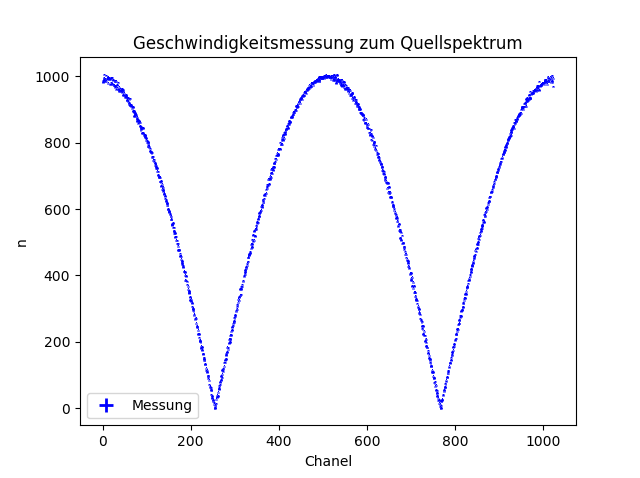
\includegraphics[scale=0.8]{Bilder/Kalibration/Quellspektrum_rohdaten.png}
\caption{Aufnahme zur Geschwindigkeits- und Energiekalibration vor der Messung des Quellspektrums.}
\label{fig:KalibrationRohdaten_Beispiel}
\end{figure}

\begin{table}
\centering
\begin{tabular}{|c|c|c|}
\hline 
Messung & Nulldurchgang 1 [ch] & Nulldurchgang 2 [ch] \\ 
\hline 
Extinktionswirkungsquerschnitt & 255 & 767 \\
\hline 
Quellspektrum & 255 & 767 \\
\hline 
Einlinienspektrum & 256 & 766 \\
\hline 
Hyperfeinstrukturaufspaltung & 255 & 766 \\
\hline 
Quadrupolaufspaltung & 255 & 767 \\
\hline 
\end{tabular} 
\caption{Abgelesene Nulldurchgänge bei den Geschwindigkeitsmessungen.}
\label{tab:Kalibration_Nulldurchgänge}
\end{table}

Abbildung \ref{fig:KalibrationRohdaten_Beispiel} zeigt beispielhaft das Messergebnis zur Geschwindigkeitsmessung. Da der Transducer die Quelle sinusförmig bewegt und die Messung der Hell-Dunkel-Übergänge nur Beträge und keine Vorzeichen misst, handelt es sich um eine Kosinus-Betragsfunktion. Für die Kalibration wird allerdings die reine Kosinusfunktion benötigt, daher werden die Daten zwischen den Nulldurchgängen mit (-1) multipliziert. Die zu diesem Zweck abgelesenen Nulldurchgänge sind in Tabelle \ref{tab:Kalibration_Nulldurchgänge} aufgelistet. \\
An die so korrigierten Daten wird dann eine Kosinusfunktion der Form
\begin{equation*}
n(\textrm{ch}) = A \cdot \cos (\omega \cdot \textrm{ch})
\end{equation*}
angepasst. Als Fehler für die Anpassung wurde für die Kanalaufteilung eine Gleichverteilung zwischen den Kanälen angenommen. Für den Fehler auf die counts wurde ein möglichst kleiner Wert verwendet, für den der Fit immer noch stabil ist. Für die Anpassungen wurden daher folgende Fehler verwendet:
\begin{equation*}
\sigma _{counts} = 2
\end{equation*}
\begin{equation*}
\sigma _\textrm{ch} = \dfrac{1}{\sqrt{12}}
\end{equation*}
Die korrigierten Daten und die Anpassung sind für dasselbe Beispiel in Abbildung \ref{fig:Kalibration_Beispiel} gezeigt. Die Ergebnisse der Anpassungen sind in Tabelle \ref{tab:Kalibration_Fitergebnisse} dargestellt. \\
Aus der Anpassung kann die dem Kanal zugehörige Momentangeschwindigkeit und daraus mit dem Dopplereffekt die Energie bestimmt werden:
\begin{equation*}
v(\textrm{ch}) = \dfrac{n(\textrm{ch}) \cdot 1024}{3160.56 \cdot t \textrm{[s]}} \textrm{[mm/s]}
\end{equation*}
\begin{equation*}
E(v) = E_0 \cdot \left(1 + \dfrac{v}{c}\right)
\end{equation*}
Wobei $E_0 = \SI{14,4}{keV}$ die Energie der verwendeten Linie ist.

\begin{table}
\centering
\begin{tabular}{|c|c|c|c|}
\hline 
Messung & Amplitude A & Frequenz $\omega$ & $\chi ^2$/ndof \\ 
\hline 
Extinktionswirkungsquerschnitt & 1053,28 $\pm$ 0,30 & 0,00615017 $\pm$ 5,7 $\cdot 10^{-7}$ & 9,394  \\
\hline 
Quellspektrum & 994,96 $\pm$ 0,29 & 0,00615257 $\pm$ 5,8 $\cdot 10^{-7}$ & 8,918 \\
\hline 
Einlinienspektrum & 387,30 $\pm$ 0,22 & 0,0061532 $\pm$ 1,0 $\cdot 10^{-6}$ & 5,768  \\
\hline 
Hyperfeinstrukturaufspaltung & 790,01 $\pm$ 0,29 & 0,00615317 $\pm$ 7,0 $\cdot 10^{-7}$ & 9,554  \\
\hline 
Quadrupolaufspaltung & 471,48 $\pm$ 0,18 & 0,00615197 $\pm$ 6,8 $\cdot 10^{-7}$ & 3,835 \\
\hline 
\end{tabular} 
\caption{Ergebnisse der Anpassungen an die Daten der Kalibrationsmessungen.}
\label{tab:Kalibration_Fitergebnisse}
\end{table}

\begin{figure}
\centering
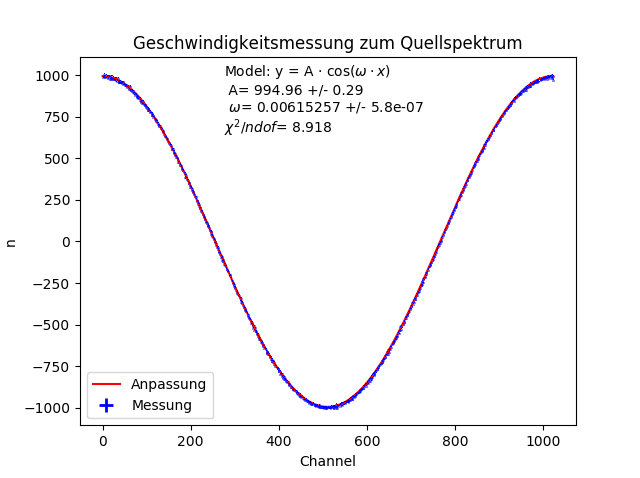
\includegraphics[scale=0.8]{Bilder/Kalibration/Quellspektrum.png}
\caption{Aufnahme zur Geschwindigkeits- und Energiekalibration vor der Messung des Quellspektrums.}
\label{fig:Kalibration_Beispiel}
\end{figure}

\subsection{Rauschmessung}
\begin{figure}
\centering
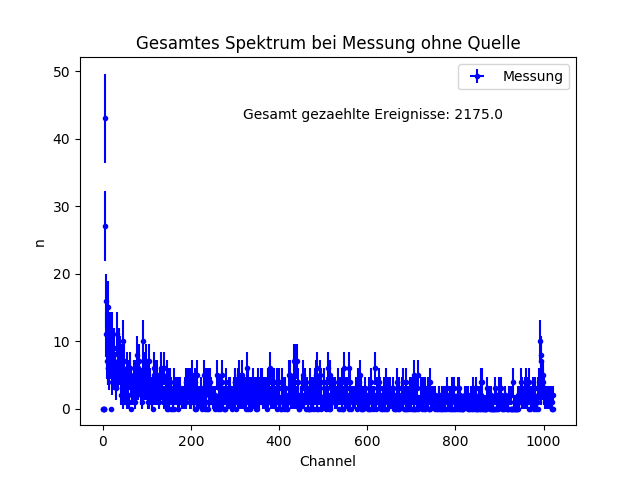
\includegraphics[scale=0.8]{Bilder/Extinktion/Rauschmessung.png}
\caption{Rauschmessung ohne Quelle und ohne Absorber zur Korrektur bei den Messungen zum Extinktionswirkungsquerschnitt.}
\label{fig:Extinktion_Rauschmessung}
\end{figure}

Abbildung \ref{fig:Extinktion_Rauschmessung} zeigt das ohne Quelle und ohne Absorber gemessene Spektrum. Da es sich bei den gemessenen Ereignissen um Zerfälle handelt ist der Fehler darauf die Wurzel:
\begin{equation*}
\sigma _{n} = \sqrt{n}
\end{equation*}
Die Gesamtzahl der gemessenen Ereignisse ist:
\begin{equation*}
Z_{Rauschen} = \dfrac{2175 \pm 46,6}{\SI{10}{min}}
\end{equation*}

\subsection{Extinktionswirkungsquerschnitt}
\begin{figure}
\centering
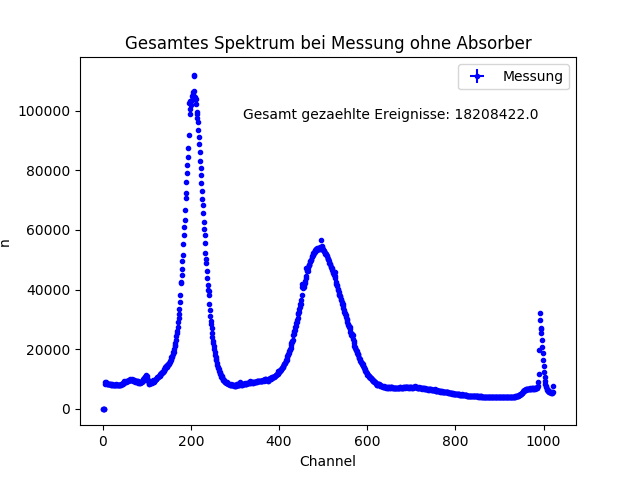
\includegraphics[scale=0.8]{Bilder/Extinktion/OhneAbsorber.png}
\caption{Messung ohne Absorber zur Bestimmung des Extinktionswirkungsquerschnitt.}
\label{fig:Extinktion_ohneAbsorber}
\end{figure}

\begin{figure}
\centering
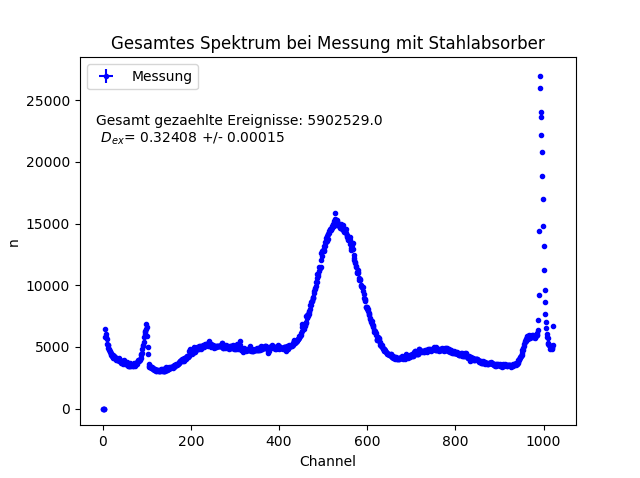
\includegraphics[scale=0.8]{Bilder/Extinktion/Stahl.png}
\caption{Messung mit Stahlabsorber zur Bestimmung des Extinktionswirkungsquerschnitts von Stahl.}
\label{fig:Extinktion_Stahl}
\end{figure}

Abbildung \ref{fig:Extinktion_ohneAbsorber} zeigt das gemessene Spektrum ohne Absorber und Abbildung \ref{fig:Extinktion_Stahl} beispielhaft für die Messung mit dem Stahlabsorber. \\
Zur Bestimmung des Extinktionswirkungsquerschnitts wird die Zählrate des gesamten Spektrums integriert bzw. wegen der Kanalauflösung aufsummiert. Auch hier wird der Fehler als 
\begin{equation*}
\sigma _{n} = \sqrt{n}
\end{equation*}
abgeschätzt. Zur Berechnung des Extinktionswirkungsquerschnitts müssen sowohl die Zählrate mit dem jeweiligen Absorber $n_A$ als auch die Zählrate ohne Absorber $n_O$ um die Untergrundmessung $n_U$ korrigiert werden, sodass sich der Extinktionswirkungsquerschnitt insgesamt bestimmt zu:
\begin{equation*}
D_{ex} = \dfrac{n_A - n_U}{n_O - n_U}
\end{equation*}
Damit bestimmt sich der Fehler mit gaußscher Fehlerfortpflanzung und der Annahme, dass die Fehler auf die Zählraten immer die Wurzel der Zählraten sind:
\begin{equation*}
\sigma _{D_{ex}} = D_{ex} \cdot \sqrt{ \left( \dfrac{\sqrt{n_O + n_U}}{n_O - n_U} \right)^2 +  \left( \dfrac{\sqrt{n_A + n_U}}{n_A - n_U} \right)^2}
\end{equation*}
Tabelle \ref{tab:Extinktion_Ergebnisse} zeigt die gemessenen Zählraten und die daraus berechneten Extinktionswirkungsquerschnitte.

\begin{table}
\centering
\begin{tabular}{|c|c|c|}
\hline 
Absorber & Zählrate $n_A$ & Extinktionswirkungsquerschnitt $D_{ex}$ \\ 
\hline 
Stahl & - & -   \\
\hline 
\end{tabular} 
\caption{Gemessene Zählraten und daraus berechnete Extinktionswirkungsquerschnitte.}
\label{tab:Extinktion_Ergebnisse}
\end{table}

\subsection{Quellenspektrum}
\subsection{Einlinienspektrum}
\subsection{Magnetische Hyperfeinstrukturaufspaltung}
\subsection{Elektrische Quadrupolaufspaltung}

\section{Fazit}


\newpage
\section{Anhang}
\subsection{Kalibration}
\begin{figure} [H]
\centering
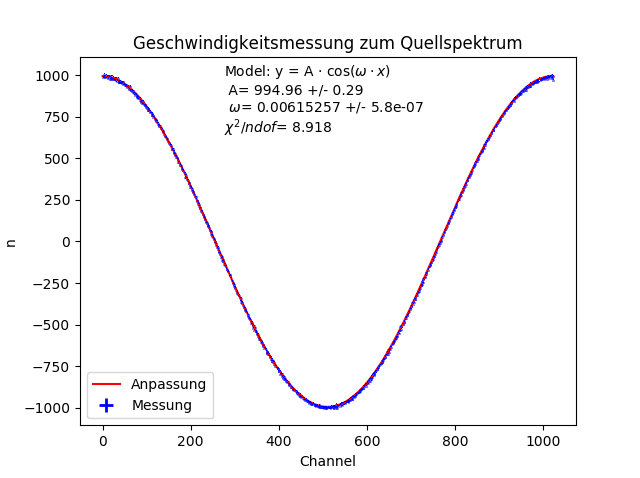
\includegraphics[scale=0.8]{Bilder/Kalibration/Quellspektrum.png}
\caption{Aufnahme zur Geschwindigkeits- und Energiekalibration vor der Messung des Quellspektrums.}
\end{figure}

\begin{figure} [H]
\centering
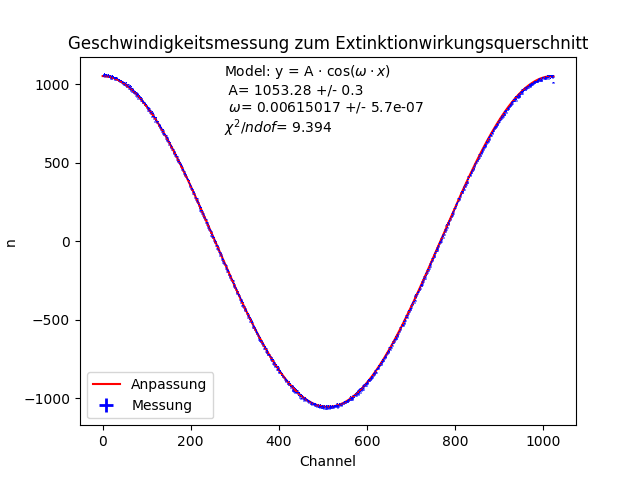
\includegraphics[scale=0.8]{Bilder/Kalibration/Extinktion.png}
\caption{Aufnahme zur Geschwindigkeits- und Energiekalibration vor der Messung des Extinktionswirkungsquerschnitts.}
\end{figure}

\begin{figure} [H]
\centering
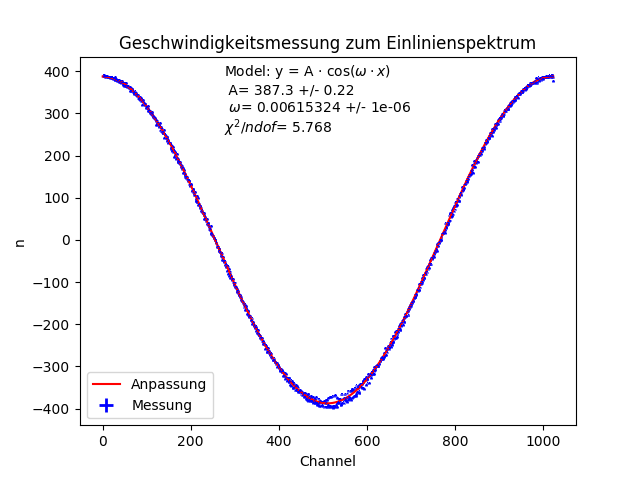
\includegraphics[scale=0.8]{Bilder/Kalibration/Einlinien.png}
\caption{Aufnahme zur Geschwindigkeits- und Energiekalibration vor der Messung des Einlinienspektrums.}
\end{figure}

\begin{figure} [H]
\centering
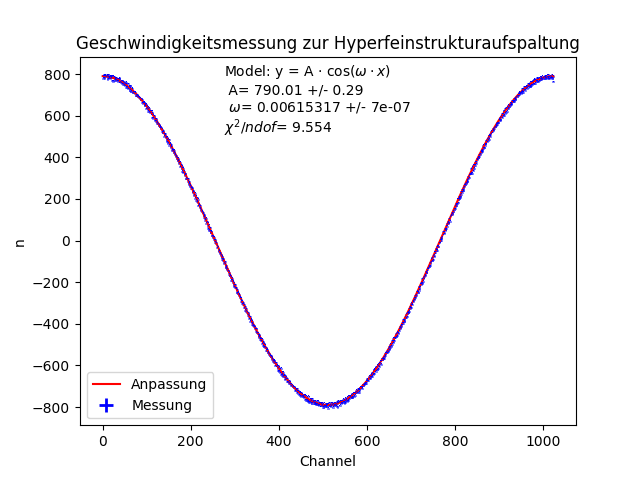
\includegraphics[scale=0.8]{Bilder/Kalibration/Hyperfein.png}
\caption{Aufnahme zur Geschwindigkeits- und Energiekalibration vor der Messung der magnetischen Hyperfeinstrukturaufspaltung.}
\end{figure}

\begin{figure} [H]
\centering
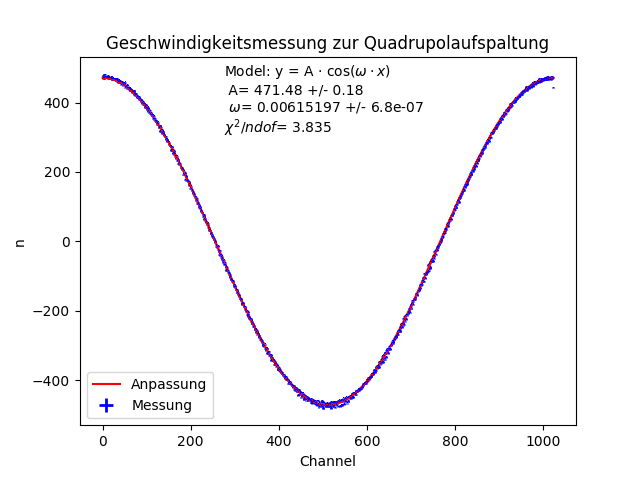
\includegraphics[scale=0.8]{Bilder/Kalibration/Quadrupol.png}
\caption{Aufnahme zur Geschwindigkeits- und Energiekalibration vor der Messung der elektrischen Quadrupolaufspaltung.}
\end{figure}

\subsection{Rauschmessung}
\begin{figure} [H]
\centering
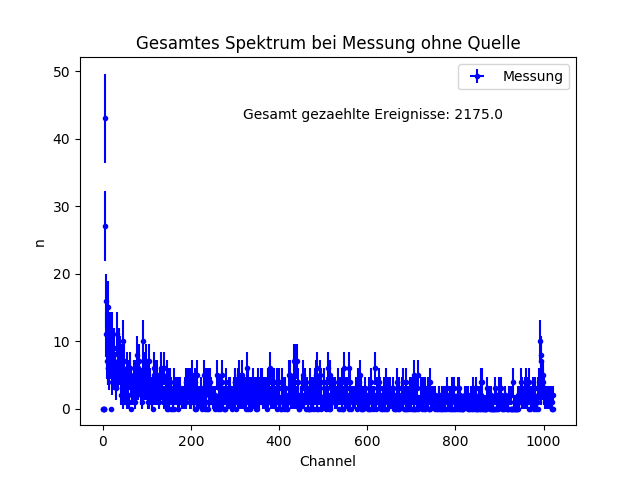
\includegraphics[scale=0.8]{Bilder/Extinktion/Rauschmessung.png}
\caption{Rauschmessung ohne Quelle und ohne Absorber zur Korrektur bei den Messungen zum Extinktionswirkungsquerschnitt.}
\end{figure}

\subsection{Extinktionswirkungsquerschnitt}
\subsection{Quellenspektrum}
\subsection{Einlinienspektrum}
\subsection{Magnetische Hyperfeinstrukturaufspaltung}
\subsection{Elektrische Quadrupolaufspaltung}


\end{document}
